\documentclass[11pt]{article}
\usepackage[BoldFont,SlantFont,CJKchecksingle]{xeCJK}
\usepackage[top=0.5in,bottom=0.5in,left=1.25in,right=0.8in]{geometry}
\setCJKmainfont[BoldFont=SimHei]{SimSun}
\setCJKmonofont{SimSun}% 设置缺省中文字体
\parindent 0em   %段首缩进
%\usepackage{indentfirst}	%设置第一段也首行缩进
\linespread{1}	%设置行距
\addtolength{\parskip}{.4em}	%增加段间距0.4em
\usepackage{amsmath} % 插入数学公式
\usepackage[colorlinks,linkcolor=blue]{hyperref} 	%设置超链接

% 设置页眉页脚
\usepackage{fancyhdr}
\pagestyle{fancy}
\lhead{} 
\chead{} 
\rhead{\bfseries {ramayzhu0625@gmail.com}} 
\lfoot{} 
\cfoot{}
\rfoot{\thepage} 
\renewcommand{\headrulewidth}{0.4pt} 
\renewcommand{\footrulewidth}{0.4pt}

% \includegraphics[width = .8\textwidth]{pic.png}  图片的宽度会被缩放至页面宽度的百分之八十,图片的总高度会按比例缩放 

\begin{document}
	\title{Machine Learning Week-5}
	\author{ramay7}
	
	\maketitle % 显示标题
	\tableofcontents % 生成目录
	%\newpage
	
	\section{Evaluating a Learning Algorithm}
	
		\subsection{Evaluating a Hypothesis}
		
		A hypothesis may have a low error for the training examples but still be inaccurate (because of overfitting). Thus, to evaluate a hypothesis, given a dataset of training examples, we can split up the data into two sets: a \textbf{training set} and a \textbf{test set}. Typically, the training set consists of 70\% of your data and the test set is the remaining 30\%.
		
		The new procedure using these two sets is then:
		\begin{enumerate}
			\item Learn $\Theta$ and minimize $J_{train}(\Theta)$ using the training set
			\item Compute the test set error $J_{test}(\Theta)$
		\end{enumerate}
		
		\subsection{Model Selection and Train/Validation/Test Sets}
		One way to break down our dataset into the three sets is:
		\begin{itemize}
			\item Training set: 60\%
			\item Cross validation set: 20\%
			\item Test set: 20\%
		\end{itemize}
		
		We can now calculate three separate error values for the three different sets using the following method:
		\begin{enumerate}
			\item Optimize the parameters in $\Theta$ using the training set for each polynomial degree.
			\item Find the polynomial degree $d$ with the least error using the cross validation set.
			\item Estimate the generalization error using the test set with $J_{test}(\Theta^{(d)})$, (d = theta from polynomial with lower error);
		\end{enumerate}
		This way, the degree of the polynomial d has not been trained using the test set.
	
	\section{Bias vs Variance}
	
		In order to choose the model and the regularization term $\lambda$, we need to:
	
		\begin{itemize}
			\item Create a list of lambdas (i.e. $\lambda \in\{0,0.01,0.02,0.04,0.08,0.16,0.32,0.64,1.28,2.56,5.12,10.24\})$;
			\item Create a set of models with different degrees or any other variants.
			\item Iterate through the $\lambda$s and for each $\lambda$ go through all the models to learn some $\Theta$.
			\item Compute the cross validation error using the learned $\Theta$ (computed with $\lambda$) on the $J_{CV}(\Theta)$ without regularization or $\lambda$ = 0.
			\item Select the best combo that produces the lowest error on the cross validation set.
			\item Using the best combo $\Theta$ and $\lambda$, apply it on $J_{test}(\Theta)$ to see if it has a good generalization of the problem.
		\end{itemize}
		
		\subsection{Learning Curves}
			Experiencing \textbf{high bias}:
			
			
			\textbf{Low training set size}: causes $J_{train}(\Theta)$ to be low and $J_{CV}(\Theta)$ to be high.
		
			\textbf{Large training set size}: causes both $J_{train}(\Theta)$ and $J_{CV}(\Theta)$ to be high with Jtrain(Θ)≈JCV(Θ).
		
			If a learning algorithm is suffering from high bias, getting more training data will \textbf{not (by itself) help much}.	
			
			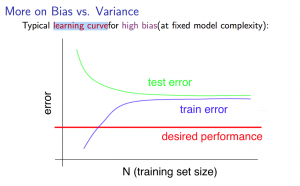
\includegraphics{high_bias.png}
			
			Experiencing \textbf{high variance}:
			
			\textbf{Low training set size}: $J_{train}(\Theta)$ will be low and $J_{CV}(\Theta)$ will be high.
			
			\textbf{Large training set siz}e: $J_{train}(\Theta)$ increases with training set size and $J_{CV}(\Theta)$ continues to decrease without leveling off. Also, $J_{train}(\Theta)$ < $J_{CV}(\Theta)$ but the difference between them remains significant.
			
			If a learning algorithm is suffering from high variance, getting more training data \textbf{is likely to help}.
			
			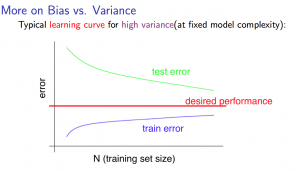
\includegraphics{high_variance}
		
		\subsection{Deciding What to Do Next Revisited}
		
			Our decision process can be broken down as follows:
		
			\begin{itemize}
				\item \textbf{Getting more training examples}: Fixes high variance
				\item \textbf{Trying smaller sets of features}: Fixes high variance
				\item \textbf{Adding features}: Fixes high bias
				\item \textbf{Adding polynomial features}: Fixes high bias
				\item \textbf{Decreasing $\lambda$}: Fixes high bias
				\item \textbf{Increasing $\lambda$}: Fixes high variance.
			\end{itemize}

\end{document}